% figure1_whyhow.tex — Why-and-How Pair (a)(b).
% (a) Quantitative gap: compress-only vs RepairKV on a tiny accuracy-vs-K curve
%     with a callout for the key result at K=96.
% (b) Mechanism strip: GPU lane on top, Host lane on bottom, three
%     phase-stages (compress / idle scan / promote) connecting them.
% Shared preamble for standalone Figure 1 variants.
\documentclass[border=8pt,tikz]{standalone}
\usepackage{amsmath}
\usepackage{amssymb}
\usepackage{tikz}
\usetikzlibrary{arrows.meta,positioning,calc,fit,shapes.geometric,backgrounds}
\usepackage{xcolor}
\usepackage[T1]{fontenc}
\usepackage{mathptmx}
\newcommand{\repairkv}{\textsc{RepairKV}}
\newcommand{\bbase}{\ensuremath{B_{\mathrm{base}}}}
\newcommand{\bmatch}{\ensuremath{B_{\mathrm{match}}}}

\begin{document}
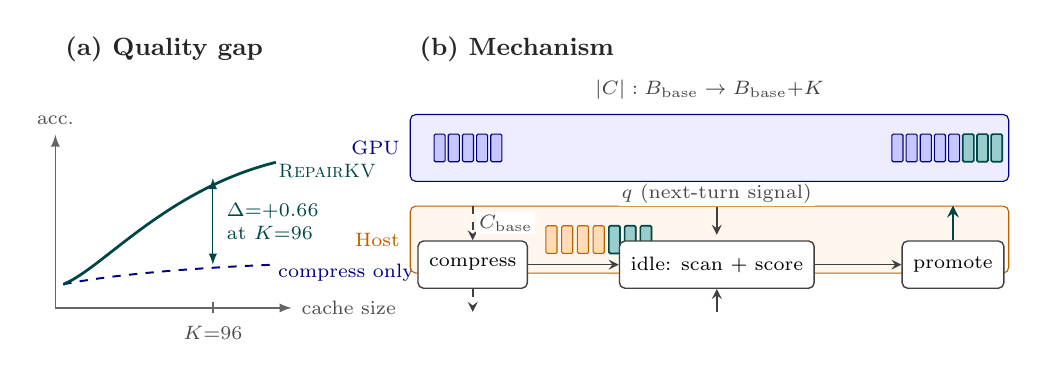
\begin{tikzpicture}[
  >=latex, line width=0.5pt,
  font=\small,
  % Panel (a) styles
  axis/.style={draw=black!60, line width=0.5pt, >=latex},
  curveR/.style={draw=teal!55!black, line width=1pt},
  curveB/.style={draw=blue!50!black, line width=0.7pt, dashed},
  panellabel/.style={font=\bfseries\small, text=black!85},
  axislabel/.style={font=\scriptsize, text=black!70},
  callout/.style={font=\scriptsize, text=teal!55!black, align=left},
  % Panel (b) styles
  lane/.style={rounded corners=2pt, line width=0.4pt, minimum height=0.85cm},
  gpulane/.style={lane, draw=blue!50!black, fill=blue!7},
  hostlane/.style={lane, draw=orange!75!black, fill=orange!7},
  stagebox/.style={draw=black!75, fill=white, line width=0.5pt,
                   inner sep=4pt, align=center, font=\scriptsize,
                   rounded corners=2pt, minimum height=0.6cm},
  active/.style={stagebox, fill=blue!12, draw=blue!55!black, line width=0.7pt},
  chip/.style={rounded corners=0.5pt, minimum width=4pt, minimum height=10pt,
               inner sep=0pt, line width=0.4pt},
  gpuchip/.style={chip, draw=blue!50!black, fill=blue!22},
  hostchip/.style={chip, draw=orange!75!black, fill=orange!28},
  promchip/.style={chip, draw=teal!55!black, fill=teal!40, line width=0.6pt},
  arr/.style={->, line width=0.6pt, draw=black!75, >=stealth},
  promarr/.style={->, line width=0.9pt, draw=teal!55!black, >=stealth},
  arrlabel/.style={font=\scriptsize, fill=white, inner sep=1pt, text=black!72}
]
  % =============================================================
  % Panel (a) — Why: accuracy gap
  % =============================================================
  \node[panellabel, anchor=south west] at (0, 3.0) {(a) Quality gap};

  % Frame: x in [0, 3.0], y in [0, 2.0]
  \draw[axis, ->] (0, 0) -- (3.0, 0)
        node[axislabel, anchor=west] {cache size};
  \draw[axis, ->] (0, 0) -- (0, 2.2)
        node[axislabel, anchor=south] {acc.};

  % compress-only curve (flat-ish low)
  \draw[curveB] (0.1, 0.3)
        .. controls (0.6, 0.4) and (1.5, 0.5) ..
        (2.8, 0.55) node[axislabel, text=blue!50!black, anchor=west, xshift=-0.1cm, yshift=-3pt] {compress only};

  % RepairKV curve (higher, climbing)
  \draw[curveR] (0.1, 0.3)
        .. controls (0.6, 0.5) and (1.4, 1.5) ..
        (2.8, 1.85) node[callout, anchor=west, xshift=-0.1cm, yshift=-3pt] {\repairkv{}};

  % Gap arrow + callout at K=96 (x=2.0)
  \draw[<->, line width=0.4pt, draw=teal!55!black]
        (2.0, 0.55) -- (2.0, 1.65);
  \node[callout, anchor=west] at (2.05, 1.1)
        {$\Delta{=}{+}0.66$\\at $K{=}96$};

  % Bottom x-axis tick at K=96
  \draw[axis] (2.0, -2pt) -- (2.0, 2pt);
  \node[axislabel, anchor=north] at (2.0, -3pt) {$K{=}96$};

  % =============================================================
  % Panel (b) — How: mechanism strip
  % =============================================================
  \node[panellabel, anchor=south west] at (4.5, 3.0) {(b) Mechanism};

  % GPU lane (top)
  \node[gpulane, minimum width=7.6cm, anchor=south west] (gpulane) at (4.5, 1.6) {};
  \node[axislabel, text=blue!55!black, anchor=east] at (gpulane.west) {GPU};

  % Host lane (bottom)
  \node[hostlane, minimum width=7.6cm, anchor=north west] (hostlane) at (4.5, 1.3) {};
  \node[axislabel, text=orange!75!black, anchor=east] at (hostlane.west) {Host};

  % --- Cache states inside GPU lane ---
  % Cbase (left)
  \foreach \i in {1,...,5}{
    \pgfmathsetmacro{\xc}{0.18*\i}
    \node[gpuchip] at ([xshift=\xc cm + 0.2cm]gpulane.west) {};
  }
  % Cbase+SK (right)
  \foreach \i in {1,...,5}{
    \pgfmathsetmacro{\xc}{0.18*\i}
    \node[gpuchip] at ([xshift=\xc cm - 1.6cm]gpulane.east) {};
  }
  \foreach \i in {1,2,3}{
    \pgfmathsetmacro{\xs}{0.18*5+0.18*\i}
    \node[promchip] at ([xshift=\xs cm - 1.6cm]gpulane.east) {};
  }

  % --- W_N inside Host lane ---
  \foreach \i in {1,...,7}{
    \pgfmathsetmacro{\xh}{0.20*\i}
    \node[hostchip] at ([xshift=\xh cm + 1.6cm]hostlane.west) {};
  }
  \pgfmathsetmacro{\xPa}{0.20*5}
  \pgfmathsetmacro{\xPb}{0.20*6}
  \pgfmathsetmacro{\xPc}{0.20*7}
  \node[promchip] at ([xshift=\xPa cm + 1.6cm]hostlane.west) {};
  \node[promchip] at ([xshift=\xPb cm + 1.6cm]hostlane.west) {};
  \node[promchip] at ([xshift=\xPc cm + 1.6cm]hostlane.west) {};

  % --- Phase stages (across the lane gap, in 3 columns) ---
  % column 1: compress
  \node[stagebox, anchor=center] (sCompress) at (5.3, 0.55) {compress};
  % column 2: idle scan + score
  \node[stagebox, anchor=center, minimum width=2.0cm] (sIdle) at (8.4, 0.55) {idle: scan + score};
  % column 3: promote
  \node[stagebox, anchor=center] (sPromote) at (11.4, 0.55) {promote};

  % Phase stage arrows (sequential)
  \draw[arr] (sCompress) -- (sIdle);
  \draw[arr] (sIdle) -- (sPromote);

  % q (next-turn signal) entering idle stage from above
  \draw[arr] ([yshift=12pt]sIdle.north) -- ([yshift=2pt]sIdle.north);
  \node[arrlabel, anchor=south] at ([yshift=12pt]sIdle.north)
       {$q$ (next-turn signal)};

  % Vertical connectors GPU <-> stages <-> Host
  \draw[arr, dashed] (5.3, 1.3) -- (sCompress.north)
       node[arrlabel, midway, right=1pt] {$C_{\mathrm{base}}$};
  \draw[arr, dashed] (sCompress.south) -- (5.3, -0.05);
  % score reads host
  \draw[arr] (8.4, -0.05) -- (sIdle.south);
  % promote -> GPU
  \draw[promarr] (sPromote.north) -- (11.4, 1.3);

  % --- Cache size growth tag ---
  \node[arrlabel, anchor=south, text=black!75]
       at ([yshift=4pt]gpulane.north) {$|C|: \bbase \to \bbase{+}K$};
\end{tikzpicture}
\end{document}
